\chapter{}\label{chap:appendix_distRL}
\section{Distributional RL} 

In contrast to standard RL, where we model the expected return, in distributional RL, we aim
to model the full distribution of the return, i.e the \textit{value distribution}.
\citet{Bellemare2017,Dabney2018a,Dabney2018b} presented different algorithms for distributional RL
and they argued the advantages of learning the whole distribution
even when we want to optimize the expected value, as the distribution can give us more information that
can be beneficial to learn function approximations.
Its advantage becomes more obvious when designing risk-sensitive algorithms that aim 
to reduce probability of
certain outcomes.

\subsection{Distributional Bellman Operator $\mathcal{T}^\pi$}

We define the random return $Z^\pi(x,a)$ as the random variable that represents the sum
of discounted rewards
obtained by 
starting from position \textit{x} taking action \textit{a} and thereupon following
policy $\pi$.
This variable captures intrinsic randomness from: immediate rewards, stochastic dynamics
and possibly an stochastic policy.
It follows:
\begin{equation}
    Q^\pi(x,a) = \mathbb E[Z^\pi(x,a)]
\end{equation}

Similarly than Q-value \ref{eq:bellman1}, Z is also described by a recursive equation, 
but of a distributional nature: 
\begin{eqnarray}
    Z^\pi(x,a) \stackrel{D}{=} R(x,a) + \gamma Z(x',a') \label{eq:distrbellman}
\end{eqnarray}
where $x'\backsim\ p(\cdot|x,a) \text{ and } a' \backsim\ \pi(\cdot |x')$ and $\stackrel{D}{=}$ 
denotes that the RV on both sides of the equation share the same
probability distribution.\\
The \textit{distributional Bellman equation} defined in \eqref{eq:distrbellman}, states
that the distribution of 
Z is characterized by the interaction of 3 random variables, the random reward R, the next
state-action (x',a') and its random return 
Z(x',a'). From here on, we will view $Z^\pi$ as a mapping from state-action pairs to
distributions over
returns, and we call this distribution the \textit{value distribution}.

In the policy evaluation setting \cite{Sutton1998}, one aims to find the value $V^\pi(x)$ or $Q^\pi(x,a)$ 
function associated with a given fixed policy $\pi$. In the distributional case, we aim to find $Z^\pi$.

We view the reward function as a random vector R $\in \mathbb{Z}$ and define the transition
operator 
$P^\pi: \mathbb{Z} $ \ra $\mathbb{Z}$
\begin{eqnarray}
    P^\pi Z(x,a) \stackrel{D}{=} Z(X',A')\\
    X'\backsim\ P(\cdot|x,a) \text{ and } A' \backsim\ \pi(\cdot |X')
\end{eqnarray}
where we use capital letters to emphasize the random nature of the next state-action pair
 (X',A').\\
\cite{Bellemare2017} defined the Distributional Bellman operator $T^\pi$ as:
\begin{eqnarray}
    T^\pi Z(x,a) \stackrel{D}{=} R(x,a) + \gamma P^\pi Z(x,a) \label{eq:distrbellmanoperator}
\end{eqnarray}
\cite{Bellemare2017} showed that \eqref{eq:distrbellmanoperator} is a contraction
mapping in Wasserstein metric whose unique fixed point is the 
random return $Z^\pi$.

\subsubsection{Wasserstein metric:}
The p-Wasserstein metric $W_p$, for $p \in [1,\infty]$, also known as the Earth Mover's 
Distance when $p=1$, is an integral probability metric between distributions. The
p-Wasserstein distance is characterized 
as the $L^p $ metric on inverse cumulative distribution functions. That is, the
p-Wasserstein metric between distributions $U $ and $Y $ is given by:
\begin{equation}
    W_p(U,Y) = \big (  \int_{0}^{1} | F_Y^{-1}(w) - F_U^{-1}(w) |^p dw   \big )^{\frac{1}{p}} \label{eq:wasserstein}
\end{equation}

where for a random variable Y, the inverse CDF $F_Y^{-1}$ of Y is defined by:
\begin{equation}
    F_Y^{-1}(w) \coloneqq \text{inf} \big\{ y \in \mathbb{R} \; | w \; \leq   F_Y(w)    \big\}
\end{equation}
where $F_Y(w) = Pr(y \leq Y)$. \\
\ref{eq:wasserstein} shows that the Wasserstein metric is the integral over the difference in the quantile functions 
of the random variables U and Y.
\ref{fig:wasserstein} illustrates the 1-Wasserstein distance as the area between two cumulative distribution
functions.
Unlike the Kullback-Leibler divergence , the Wasserstein metric is a true probability
metric and considers both the probability of
and the distance between various outcome events, which makes it well-suited to domains 
where an underlying similarity in outcome is more important than exactly matching likelihoods.

\begin{figure}[ht]
    \centering
    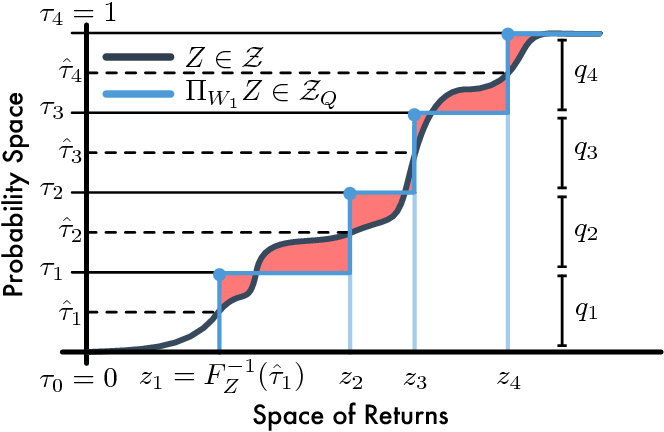
\includegraphics[width=0.8\textwidth]{images/wasserstein.png}
    \caption{Illustration of 1-Wasserstein distance as the area between 2 cumulative distribution
    functions.Shaded regions sum to form the 1-Wasserstein error. Source: \citet{Dabney2018a}}
    \label{fig:wasserstein}

\end{figure}

\subsubsection{Contraction in $\hat{d}_p$:}
Consider the process $Z_{k+1} \coloneqq T^\pi Z_{k}$, starting with some $Z_{0} \in \mathcal{Z}$, 
where $\mathcal{Z}$  is the space of action-value distributions with bounded moments.\\
\cite{Bellemare2017} showed that
$T^\pi Z: \mathcal{Z}$  \ra $\mathcal{Z}$ is a $\gamma$-contraction in the maximal form of the Wasserstein
metric $\hat{d}_p$ defined as
\begin{equation}
    \hat{d}_p(Z_1,Z_2) \coloneqq \underset{x,a} {\text{sup}}  \;W_p(Z_1(x,a),Z_2(x,a))
\end{equation}
i.e. for any two $Z_1, Z_2 \in \mathcal{Z}$,
\begin{equation}
    \hat{d}_p(T^\pi Z_1, T^\pi Z_2) \leq \gamma \hat{d}_p(Z_1,Z_2)
\end{equation}

Using Banach's fixed point theorem, we can conclude that $T^\pi$ has a unique fixed point,
which by inspection must be $Z^\pi$.

Hence the $\hat{d}_p$ metric is shown to be useful metric for studying behavior of
distributional RL algorithms, and to showed their convergence to a fixed point.
Moreover, shows than en effective way to learn a value distribution is to attempt minimize
the Wasserstein distance between a distribution Z and its distributional Bellman update
$T^\pi Z$, analogously to the way that TD-learning attempts to iteratively minimize
the $L^2$ distance between Q and $TQ$.

\subsection{Distributional Bellman Optimality Operator $\mathcal{T}$}
We have so far considered a policy evaluation setting and we studied
the behavior of its associated distributional operator $T^\pi$.
We now move to the control setting, where we aim to find a policy $\pi^{*}$ that optimizes the value and the 
corresponding distribution.

While all optimal policies attain the same value $Q^{*}$, in general there are
many optimal value distributions.
We will call a \textit{distributional Bellman optimality operator} any operator $\mathcal{T}$ 
which implements a greedy selection
rule, i.e.:
\begin{equation*}
    \mathcal{T}Z = \big\{ \mathcal{T}^\pi Z \; \text{for some}\; \pi \in   \mathcal{G_Z} \big\}
\end{equation*}
where $\mathcal{G_Z}$ is the set of greedy policies for Z, i.e. set of policies that maximize
the expectation of Z.

As in the policy evaluation setting, we are interested in the behavior of the iterates 
$Z_{k+1} := \mathcal{T}Z_k, Z_0 \in \mathcal{Z}$.
\citet{Bellemare2017} shows that the distributional analogue of the Bellman optimality operator converges, in a weak sense,
to the set of optimal value distributions, but
this operator is \textit{not a contraction in any metric between distributions.}.\\

Another result, shows that we cannot in general minimize the Wasserstein metric, 
viewed as a loss, using stochastic gradient descent methods. This limitation, is crucial
in a practical context, when the value distribution needs to be approximated.

\subsection{Quantile approximation}
\cite{Dabney2018a} used the theory of quantile regression \cite{koenker2005}, to
design an algorithm applicable in a stochastic approximation setting.
Quantile regression is used to estimate the quantile function at precisely chosen points.
Then the Bellman update is applied onto this parameterized quantile distribution.
This combined operator is proven to be a contraction and the estimated quantile function
is shown to converge to the true value distribution when minimized using stochastic approximation.

\subsubsection{Quantile projection}
We aim to estimate the quantiles of the value distribution, i.e. the values 
of the return that divide the value distribution in equally sized parts.
We call it quantile distribution.
We let $\mathcal{Z_Q}$ be the space of quantile distributions.
We denote the cumulative probabilities associated with such a distribution, known as
quantile levels, by $\tau_1,\tau_2...\tau_N$,
so that $\tau_i=\frac{i}{N}$ for $i=1,...N$.\\
Formally, let $\theta : \mathcal{X} \times \mathcal{A} \ra \mathbb R^N $ be some parametric model.
A quantile distribution $Z_\theta \in \mathcal{Z_Q}$ maps each state-action pair (x,a) to a uniform
probability distribution supported on $\{\theta_i(x,a)  \}$. Hence we can approximate it by a 
uniform mixture of N Diracs:
\begin{equation}
    Z_\theta(x,a) \coloneqq \frac{1}{N}\sum_{i=1}^{N}\delta_{\theta_i(x,a)}  \label{eq:discrete_pdf}
\end{equation}
with each $\theta_i$ assigned a fixed quantile.\\
We aim to learn the support of these Diracs, i.e. learn $\theta_i \; \forall (i, a, x)$ triplet.
We will do it by quantifying the projection of an arbitrary value distribution $Z \in \mathcal{Z}$
onto $\mathcal{Z_Q}$, that is:

\begin{equation}
    \prod{}_{W_1} Z \coloneqq  \underset{Z_\theta \in \mathcal{Z_Q}}{\arg \min } W_1(Z,Z_\theta)
\end{equation}

This projection $\prod_ {W_1}$ is the quantile projection.
We can quantify the projection between Y and U, a uniform distribution
over N Diracs as in \eqref{eq:discrete_pdf} with support $\{\theta_1, ... \theta_N\}$ by:
\begin{equation}
    W_1(Y,U)= \sum_{i=1}^{N}\int_{\tau_{i-1}}^{\tau_i} |   F_Y^{-1}(w)-\theta_i   |dw
\end{equation}

Lemma 2 in \cite{Dabney2018a} \label{par:lemma2_dabney} shows that the set of values $\{\theta_1, ... ,\theta_N\}$ that minimize:
$W_1(Y,U)$ are given by $\theta_i = F_Y^{-1}(\hat\tau_i)$, where $\hat\tau_i=\frac{\tau_{i-1}+\tau_i}{2}$.
Figure \ref{fig:wasserstein} shows the projection $\Pi_{W_1}Z$ of the function $Z$ onto $\mathcal{Z_Q}$ minimizing
the 1-Wasserstein distance to Z.\\

\subsection{Quantile Regression}
Quantile regression is a method for approximating quantile functions of a distribution at specific points.
The quantile regression loss, for quantile $\tau \in [0,1]$, is an asymmetric convex lox function
that penalizes underestimation errors with weight $\tau$ and overestimation errors
with weight $1-\tau$. \\
For a distribution Z, and given quantile $\tau$, the value of the quantile function $F_Z^{-1}(\tau)$
may be characterized as the minimizer of the quantile regression loss:
\begin{align}
    \mathcal{L}_{QR}^{\tau}(\theta)=\mathbb E_{\hat{Z}\backsim Z}[\rho_\tau(\hat{Z}-\theta) ] \label{eq:quantile_loss}\\
    \rho_\tau(u)=u(\tau - \mathds{1}_{\{u<0\}}) \quad \forall u \in \mathbb{R} \nonumber
\end{align}
Given that the minimizer of the quantile regression loss for $\tau$ is $F_Z^{-1}(\tau)$, and 
using Lemma 2 in \cite{Dabney2018a},\ref{par:lemma2_dabney} that claims that the values 
of $\{\theta_1, ... \theta_N\}$ that minimize
 $W_1(Z,Z_\theta)$ are given by $\theta_i = F_Y^-1(\hat\tau_i)$; we have that the set of minimizing
 values $\{\theta_1, ... \theta_N\}$ for  $W_1(Z,Z_\theta)$ are the minimizers of the 
 following objective:

\begin{equation}
    \sum_{i=1}^{N} \mathbb E_{\hat{Z} \sim Z} [ \rho_{\hat\tau_i}(\hat{Z}-\theta_i)]
\end{equation}

This loss gives unbiased sample gradients and hence, we can find the minimizing $\{\theta_1, ... \theta_N\}$
by stochastic gradient descent.

\begin{figure}[ht]
    \centering
    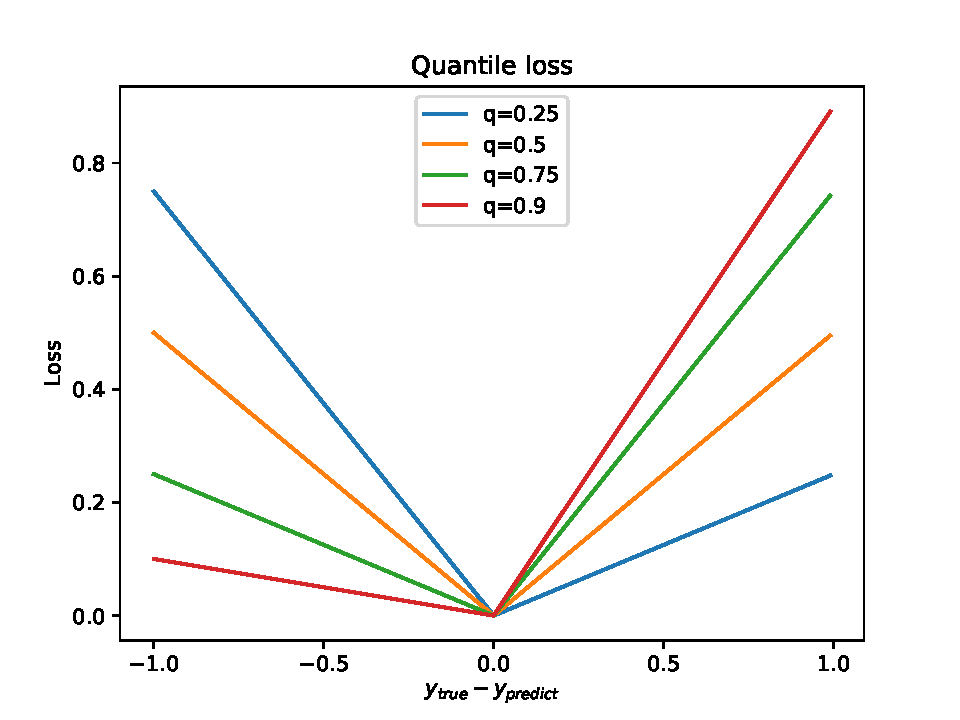
\includegraphics[width=0.8\textwidth]{images/quantile_loss.pdf}
    \caption{Quantile loss for different quantile values}
    \label{quantile_loss}
\end{figure}

Proposition 2 in \cite{Dabney2018a} states that the combined quantile projection 
$\prod_{W_1}$ with the Bellman update $\mathcal{T}^\pi$ has a unique fixed point $\hat{Z}^\pi$, and the repeated application
of this operator, or its stochastic approximation, converges to $\hat{Z}^\pi$.

\subsection{Quantile Regression Temporal Difference Learning}
Temporal difference learning updates the estimated value function with a single unbiased 
sample following policy $\pi$.
Quantile regression allows to improve the estimate of the quantile function for some target
distribution Y(x), by observing samples $y\sim Y(x)$ and minimizing equation \eqref{eq:quantile_loss}.
Using the quantile regression loss, we can obtain an approximation with minimal 1-Wasserstein distance
from the original.
We can combine this with the distributional Bellman operator to give a target distribution
for quantile regression, creating the quantile regression temporal difference learning algorithm:

\begin{eqnarray}
    u=r+\gamma z' - \theta_i(x)\\
    \theta_i(x) \la \theta_i(x) + \alpha (\hat\tau_i - \mathds{1}_{\{u<0\}})\\
    a \backsim \pi(\cdot |x) , r \backsim R(x,a), x'\backsim P(\cdot |x,a), z' \backsim Z_\theta(x')
\end{eqnarray}

where $Z_\theta$ is a quantile distribution as in \eqref{eq:discrete_pdf} and $\theta_i(x)$ 
is the estimated value of $F_{Z^\pi(x)}^{-1}(\hat\tau_i)$ in state x.


\subsection{Implicit quantile networks}
In this thesis, we represent the quantile distribution slightly different than
\eqref{eq:discrete_pdf}. We use  implicit quantile network (IQN), a deterministic
parametric function trained to reparameterize samples from a base distribution eg $\tau \in U([0,1])$ 
to the respective quantile values of a target distribution. This network is presented in \citet{Dabney2018b}.
Hence, in this case, we do not learn the distribution at uniformly separated
quantile levels $\tau_i$ ($i \in \{1,N\}$) but, the quantile level $\tau$ is now an
input to the network instead.
Despite the difference in the parameterization, approach followed is the same as described
in previous sections.\\
However, as discussed by the IQN authors \citep{Dabney2018b}, the contraction mapping
results for fixed grid of quantiles given in \citet{Dabney2018b} is not proven yet to extend 
to this more general class of approximate quantile functions.
Empirical performance success still motivates the use of the approach.\\
Curious readers are encouraged to read the papers \citet{Bellemare2017,Dabney2018a,Dabney2018b}
for more information about the distributional RL approach.

